\documentclass[12pt, a4paper]{article} 
\usepackage{tcolorbox}
\tcbuselibrary{skins, breakable, theorems}
\usepackage{subcaption}
\usepackage{pdflscape} 

\newtcbtheorem{question}{题~(理}%
  {enhanced, breakable,
    colback = white, colframe = cyan, colbacktitle = cyan,
    attach boxed title to top left = {yshift = -2mm, xshift = 5mm},
    boxed title style = {sharp corners},
    fonttitle = \sffamily\bfseries, separator sign = {).~}}{qst}
\input{pre._CJK_thesis}   % 使用自己維護的定義檔
%-----------------------------------------------------------------------------------------------------------------------
% 文章開始
\title{ Teps-b資料統計}
\author{{\SM 鄭仲恒}}
\date{{\TT \today}} 	 
\begin{document}
\maketitle
\fontsize{12}{22 pt}\selectfont
資料採用中央研究院與國立政治大學,公同主持<台灣教育長期追蹤資料庫後續調查>(TEPS-B),計畫主要探討青壯年族群從學校步入職場薪酬等議題,資料簡介:CP代表原先調查為國中生族群,SH為原先調查高中生族群。文章先由CP核心資料先介紹,後續介紹SH特性,本資料為特定受訪者的追中型資料,透過受訪者\textbf{stud-id}變數可將資料串接起,成為\textbf{panel-data}。

%%%%%%%%%%%%%%%%%%%%%%%%%%%%


\section{CP-核心資料國中生}
調查的資料分佈年份為2009、2013、2014、2019年,其中2014年度為專員實際進行面訪受訪者,其餘3次調查為電話訪談。
\subsection{2009年度調查-電訪}

\subsubsection{基本資料}
資料經處理重新標籤。保留為正式接受完電話訪談的受訪者,總計3593位,進行後需資料研究分析。性別比例男女比例近各半 表\ref{tab:gender} 呈現,受訪年紀約落於20-21歲間,此為原先樣本年紀初步估算,進步分析受訪者的科系與學校類別,表 \ref{tab:gender_school}、\ref{tab:gender_major} 得出受訪者較多較多就讀於私利大學,科系以社會科學、商學、法律最為多數。


\begin{table}[htbp]
  \centering
   \caption{受訪者性別}
  \begin{adjustbox}{width=0.5\textwidth}
    \begin{tabular}{lcccc}
      \toprule
      cp2009 & 樣本性別 & Freq. & Percent & Cum. \\
      \midrule
      & 男 & 1,764 & 49.10 & 49.10 \\
      & 女 & 1,829 & 50.90 & 100.00 \\
      \midrule
      Total & & 3,593 & 100.00 & \\
      \bottomrule
    \end{tabular}
    \label{tab:gender}
  \end{adjustbox}
\end{table}

\bigskip

\begin{table}[htbp]
  \centering
  \renewcommand{\arraystretch}{1.3} %%%把表格的高拉大
  \caption{性別與學校類別}
  \begin{adjustbox}{width=\textwidth}
    \begin{tabular}{lcccccccccc}
      \toprule
      cp2009 & 樣本性 & 大學 & 私立大學 & 國立科技 & 私立科技 & 技職學院 & 學院 & 國外大學 & 遺漏 & 跳答 \\
      \midrule
      & 男 & 424 & 528 & 100 & 256 & 150 & 16 & 9 & 178 & 103 \\
      & 女 & 350 & 639 & 77 & 247 & 162 & 8 & 25 & 230 & 91 \\
      \midrule
      Total & & 774 & 1,167 & 177 & 503 & 312 & 24 & 34 & 408 & 194 \\
      \bottomrule
    \end{tabular}
    \label{tab:gender_school}
  \end{adjustbox}
\end{table}

\bigskip

\begin{table}[H]
\centering
\extrarowheight=5pt
\caption{大學科系分析 }
\begin{adjustbox}{width=\textwidth}
\begin{tabular}{l*{7}{c}}
\toprule
 & \multicolumn{7}{c}{大學科系)} \\
gender & 教育 & 人文及藝術 & 社科、商、法 & 科學 & 工程、營造 & 農學 & 醫藥衛生 \\
 \\
\midrule
男 & 38 & 135 & 261 & 234 & 574 & 31 & 78 \\
女 & 50 & 322 & 494 & 136 & 125 & 43 & 171 \\
Total & 88 & 457 & 755 & 370 & 699 & 74 & 249 \\
\bottomrule
\label{tab:gender_major}
\end{tabular}
\end{adjustbox}
\end{table}

\begin{table}[H]
\centering
\extrarowheight=3pt
\begin{adjustbox}{width=0.8\textwidth}
\begin{tabular}{l*{7}{c}}
\toprule
cont. & 服務 & 其他 & 遺漏 & 不知道 & 拒答 & 跳答 & Total \\
\midrule
男 & 118 & 3 & 173 & 9 & 6 & 104 & 1,764 \\
女 & 158 & 3 & 224 & 8 & 2 & 93 & 1,829 \\
Total & 276 & 6 & 397 & 17 & 8 & 197 & 3,593 \\
\bottomrule
\end{tabular}
\end{adjustbox}

\end{table}





%%%%%%%%%%%%
\begin{figure}[H]
    \centering    
        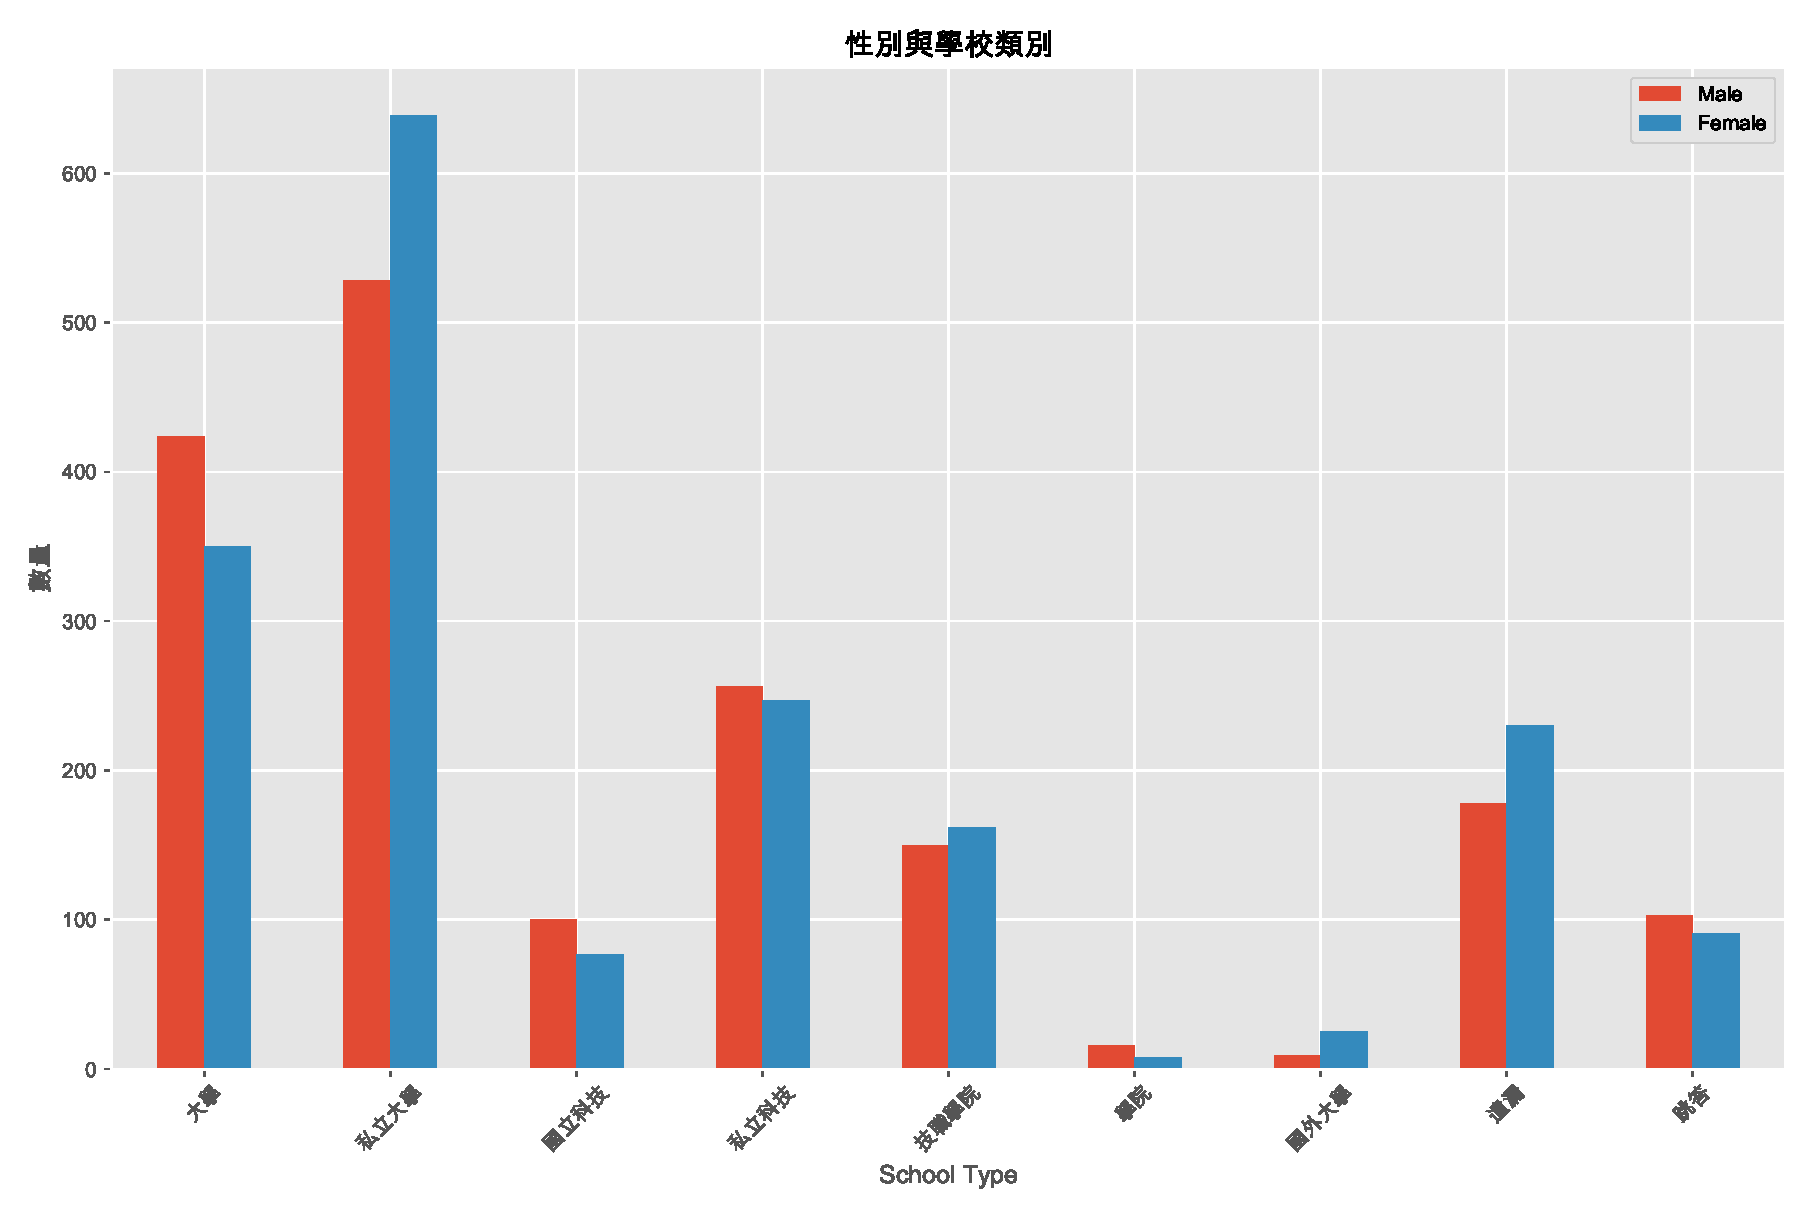
\includegraphics[width=0.9\linewidth]{\imgdir/gender_school.eps}
        \caption{學校種類與性別}
        \label{pic:shcool_gender}
\end{figure}

\begin{figure}[H]
    \centering    
        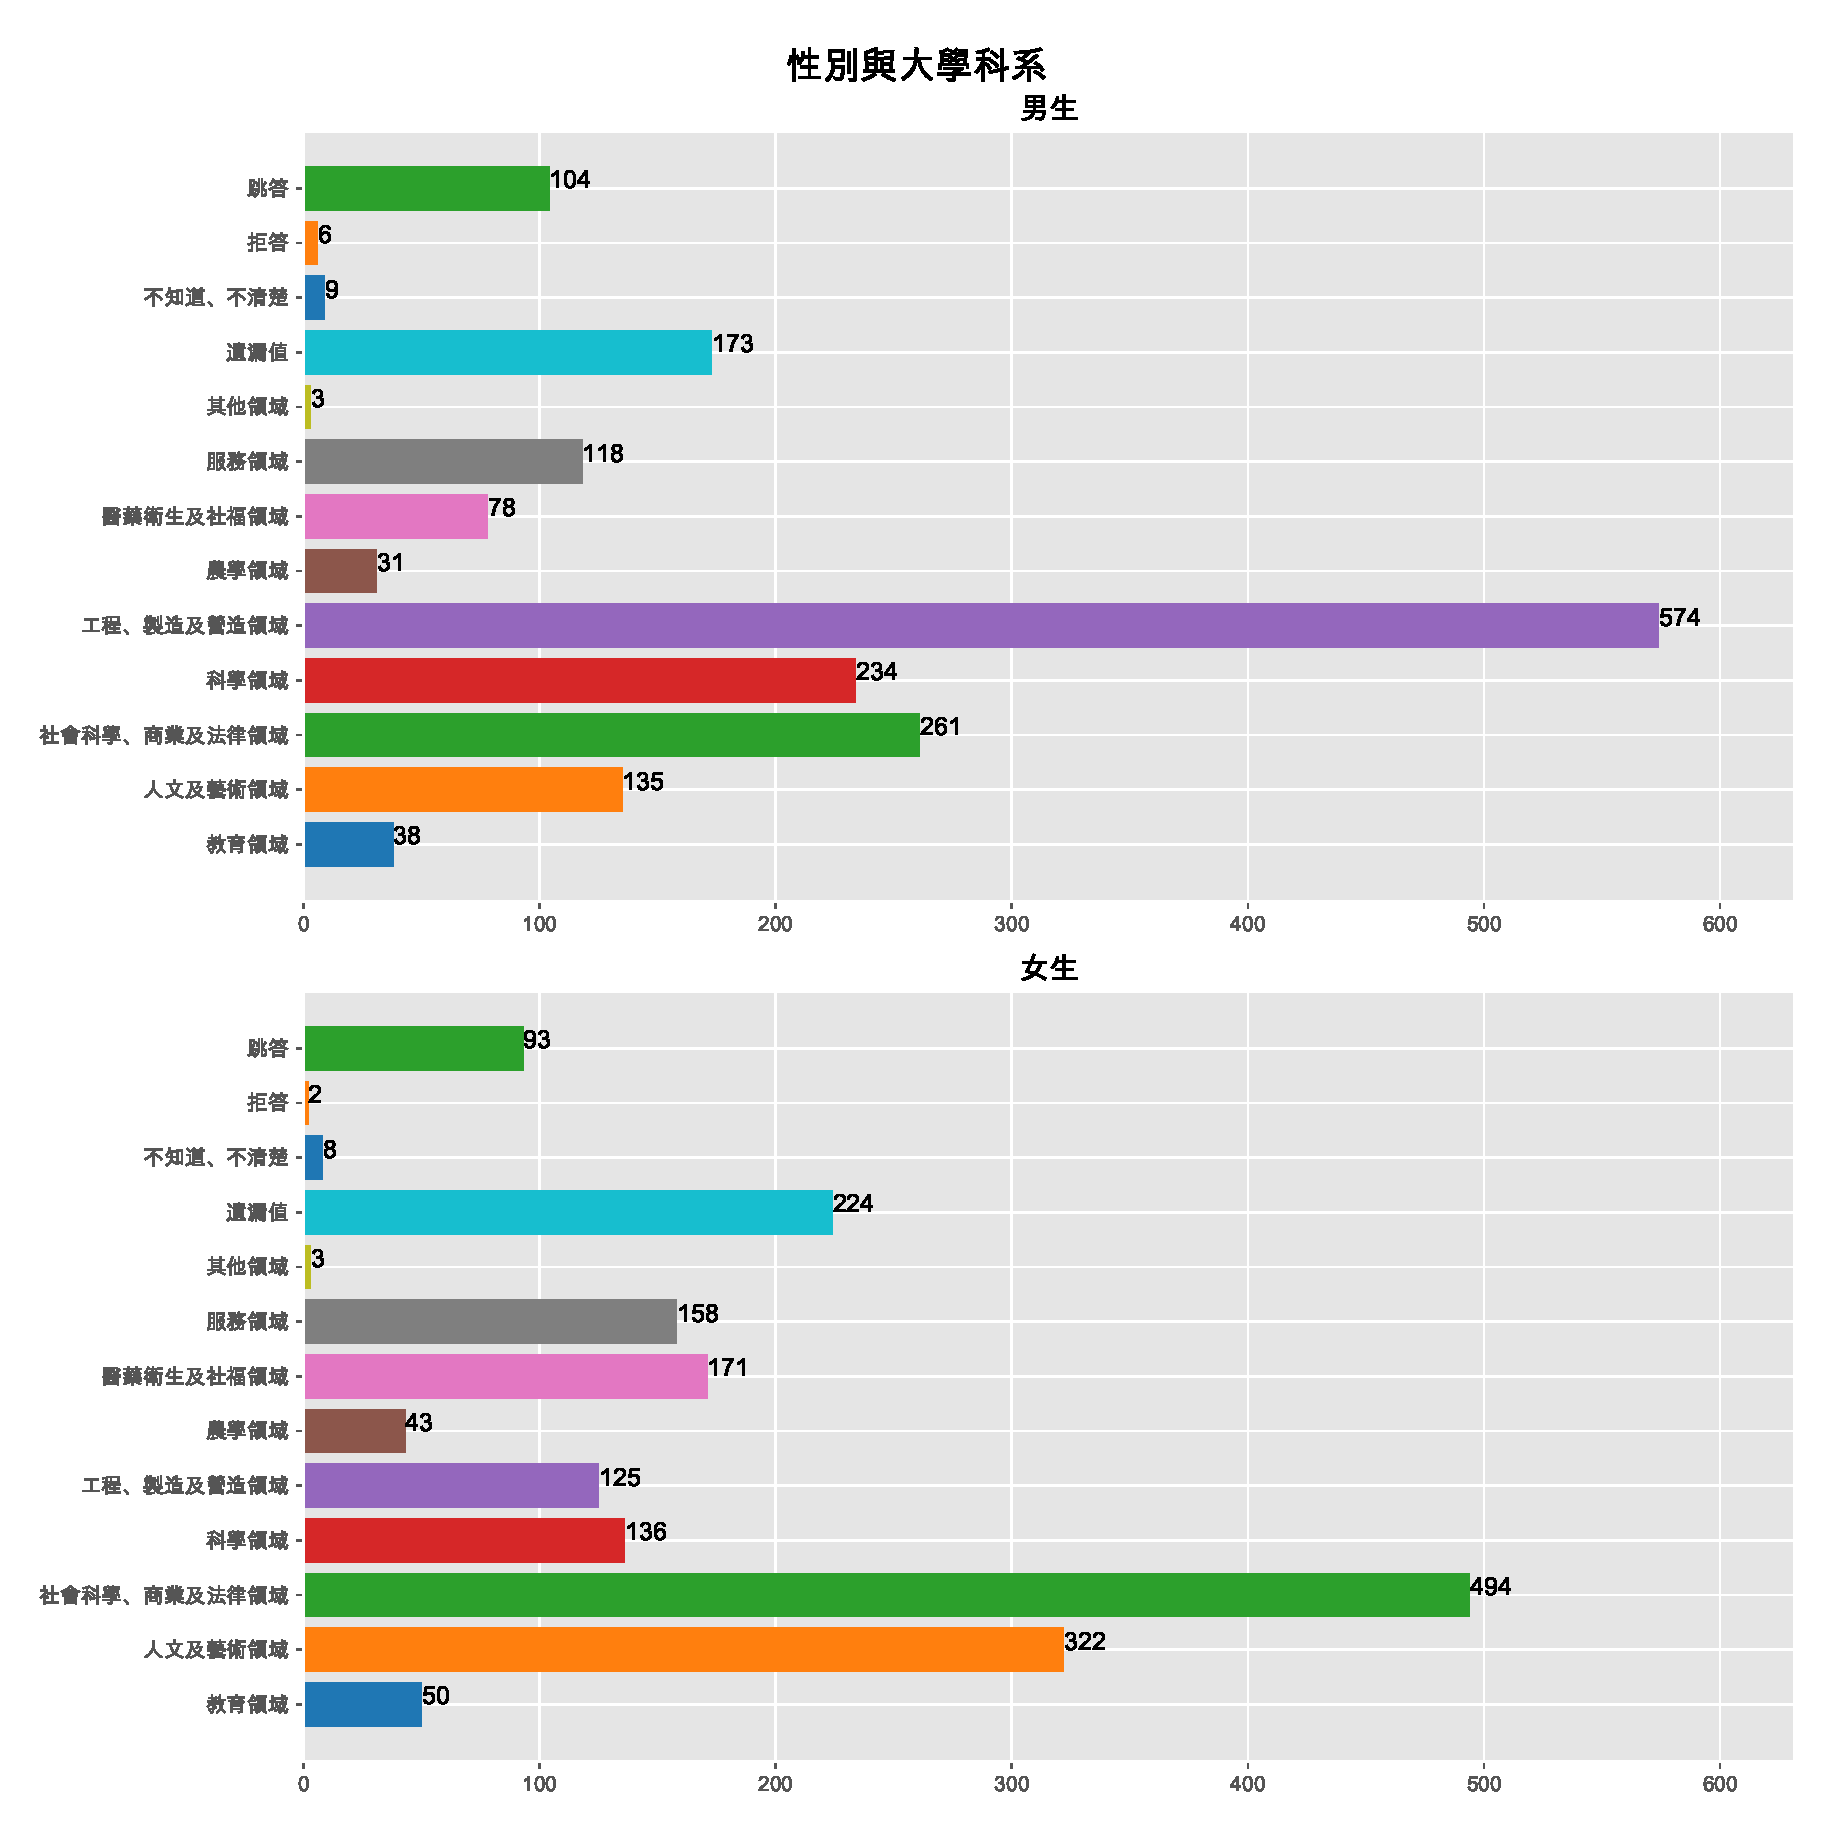
\includegraphics[width=\linewidth]{\imgdir/gender_major.eps}
        \caption{大學科科系與性別}
        \label{pic:major_gender}
\end{figure}




%%%%%%%%%%%%%%%
\clearpage
\subsubsection{學校進入職場}

從學校步入職場的分析,多數受訪於目前是否有工作、是否為第一份工作,答覆上較多資料缺失。因此在表 \ref{tab:exper_curret} 、 \ref{tab:exper_first} 較多為缺失,值得注意為受者答覆2-3幾年的工作經驗,為首次調查中最為多數,其二為私立性質院校,較多受訪者答覆有工作經驗。目前工作經驗的計算有不同,根據原始受訪問卷中問及受訪者,第一份工作和現在的工作,受訪者可能因種種因素,目前所做的工作非最初工作,約有101位答覆,工作有轉換。計算工作經驗部分暫且以兩種方是呈現。



\begin{table}[ht]
\centering
\renewcommand{\arraystretch}{1.3} %%% Adjust the row height
\extrarowheight=5pt
\caption{工作經驗(目前工作計算)}
\begin{adjustbox}{width=\textwidth}
\begin{tabular}{l*{7}{c}}
\toprule
& \multicolumn{7}{c}{工作經驗(目前工作計算)} \\
\cmidrule(lr){2-8}
\multirow{2}{*}{大學學校種類} & \multirow{2}{*}{4年-5年} & \multirow{2}{*}{3年-4年} & \multirow{2}{*}{2年-3年} & \multirow{2}{*}{1年-2年} & \multirow{2}{*}{1年內} & \multirow{2}{*}{遺漏、跳答} & \multirow{2}{*}{Total} \\
&  &  & &  & &、不清楚、跳答 &  \\
\midrule
國立大學 & 0 & 1 & 4 & 1 & 2 & 766 & 774 \\
私立大學 & 1 & 4 & 9 & 17 & 16 & 1,120 & 1,167 \\
國立科技大學 & 0 & 0 & 6 & 2 & 5 & 164 & 177 \\
私立科技大學 & 0 & 1 & 29 & 18 & 27 & 428 & 503 \\
技職學院、專科學校 & 0 & 0 & 20 & 17 & 24 & 251 & 312 \\
學院 & 0 & 0 & 0 & 1 & 0 & 23 & 24 \\
國外大學、其他 & 0 & 0 & 0 & 0 & 0 & 34 & 34 \\
遺漏、不清楚、拒答 & 0 & 0 & 1 & 0 & 1 & 406 & 408 \\
跳答 & 0 & 2 & 53 & 40 & 44 & 55 & 194 \\
Total & 1 & 8 & 122 & 96 & 119 & 3,247 & 3,593 \\
\bottomrule
\label{tab:exper_curret}
\end{tabular}
\end{adjustbox}
\end{table}

\begin{table}[H]
\centering
\renewcommand{\arraystretch}{1.3} %%%把表格的高拉大
\extrarowheight=4pt
\caption{工作經驗(第一份工作計算)}
\begin{adjustbox}{width=\textwidth}
\begin{tabular}{l*{8}{c}}
\toprule
& \multicolumn{8}{c}{工作經驗(第一份工作計算)} \\
\cmidrule(lr){2-9}
\multirow{2}{*}{大學學校種類} & \multirow{2}{*}{5年} & \multirow{2}{*}{4年-5年} & \multirow{2}{*}{3年-4年} & \multirow{2}{*}{2年-3年} & \multirow{2}{*}{1年-2年} & \multirow{2}{*}{1年內} & \multirow{2}{*}{遺漏、跳答} & \multirow{2}{*}{Total} \\
& & & & & & &、不清楚、跳答 & \\
\midrule
國立大學 & 0 & 0 & 1 & 0 & 0 & 0 & 773 & 774 \\
私立大學 & 1 & 1 & 0 & 5 & 8 & 0 & 1,152 & 1,167 \\
國立科技大學 & 0 & 0 & 0 & 0 & 1 & 0 & 176 & 177 \\
私立科技大學 & 1 & 1 & 1 & 15 & 3 & 2 & 480 & 503 \\
技職學院、專科學校 & 0 & 0 & 2 & 9 & 5 & 0 & 296 & 312 \\
學院 & 0 & 0 & 0 & 0 & 0 & 0 & 24 & 24 \\
國外大學、其他 & 0 & 0 & 0 & 0 & 0 & 0 & 34 & 34 \\
遺漏、不清楚、拒答 & 0 & 0 & 0 & 0 & 0 & 0 & 408 & 408 \\
跳答 & 0 & 0 & 3 & 25 & 4 & 3 & 159 & 194 \\
Total & 2 & 2 & 7 & 54 & 21 & 5 & 3,502 & 3,593 \\
\bottomrule
\label{tab:exper_first}
\end{tabular}
\end{adjustbox}
\end{table}


%%%%%%%%%%%%%%%%%

薪酬與學歷情況,透過
\begin{table}[ht]
\centering
\renewcommand{\arraystretch}{1.3} %%%把表格的高拉大
\extrarowheight=4pt
\caption{大學學校種類與薪酬}
\begin{adjustbox}{width=\textwidth}
\begin{tabular}{l*{8}{c}}
\toprule
& \multicolumn{8}{c}{薪酬經過重新分組} \\
\cmidrule(lr){2-9}
大學學校種類 & 2萬以下 & 2萬以上& 3萬以上 & 4萬以上 & 5萬以上 & 遺漏、 & 跳答 & Total \\
		   &    &-3萬以下    & -4萬以下  &- 5萬以下    & -6萬以下   & 不清楚、拒答   &   &  \\
\midrule
國立大學 & 5 & 3 & 0 & 0 & 0 & 3 & 763 & 774 \\
私立大學 & 28 & 17 & 2 & 0 & 0 & 2 & 1,118 & 1,167 \\
國立科技大學 & 7 & 6 & 0 & 0 & 0 & 1 & 163 & 177 \\
私立科技大學 & 46 & 24 & 4 & 0 & 0 & 6 & 423 & 503 \\
技職學院、專科學校 & 27 & 27 & 4 & 0 & 1 & 3 & 250 & 312 \\
學院 & 0 & 1 & 0 & 0 & 0 & 0 & 23 & 24 \\
國外大學、其他 & 0 & 0 & 0 & 0 & 0 & 0 & 34 & 34 \\
遺漏、不清楚、拒答 & 1 & 1 & 0 & 0 & 0 & 395 & 11 & 408 \\
跳答 & 37 & 62 & 23 & 3 & 1 & 18 & 50 & 194 \\
Total & 151 & 141 & 33 & 3 & 2 & 428 & 2,835 & 3,593 \\
\bottomrule
\label{tab:school_wage}
\end{tabular}
\end{adjustbox}
\end{table}



\begin{figure}[H]
    \centering    
        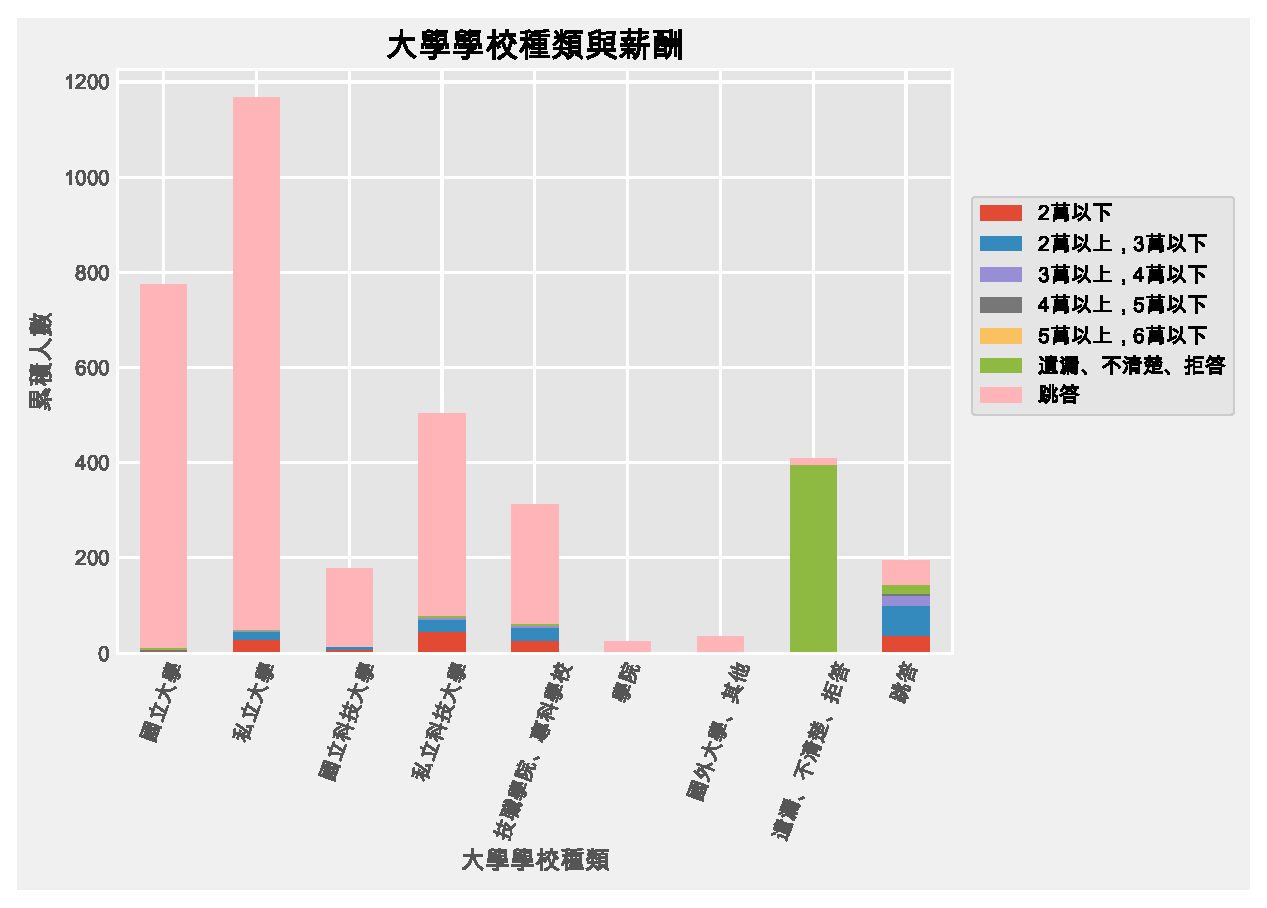
\includegraphics[width=0.9\linewidth]{\imgdir/school_type_salary.eps}
        \caption{學校種類與薪酬}
        \label{pic:school_salary}
\end{figure}



\begin{table}[ht]
\centering
\caption{變數之間的相關係數}
\begin{tabular}{lcccccc}
\toprule
& \textbf{salary\_modfy} & \textbf{gender} & \textbf{school} & \textbf{major} & \textbf{exper\_cur} & \textbf{exper} \\
\midrule
\textbf{salary\_modfy} & 1.0000 & - & - & - & - & - \\
\textbf{gender} & -0.0022 & 1.0000 & - & - & - & - \\
\textbf{school} & -0.3772 & 0.0272 & 1.0000 & - & - & - \\
\textbf{major} & -0.3187 & 0.0119 & 0.8437 & 1.0000 & - & - \\
\textbf{exper\_cur} & 0.8644 & 0.0187 & -0.2727 & -0.2004 & 1.0000 & - \\
\textbf{exper} & 0.4685 & -0.0239 & -0.1323 & -0.0925 & 0.3327 & 1.0000 \\
\bottomrule
\end{tabular}
\end{table}

\end{document}



\begin{table}






\end{document}
